% vim: set tabstop=4:
% vim: set shiftwidth=4:
% vim: set expandtab:
\RHpresentationHead{
\documentclass[pdftex,unicode,xcolor=table]{beamer}
%\documentclass[pdftex,unicode,xcolor=table,notes=show]{beamer}
}

\RHarticleHead{
% This does not work, because of colors, \insertauthor, etc.
\documentclass[a4paper,12pt,pdftex,unicode]{article}
\usepackage[envcountsect]{beamerarticle}
}

\mode<presentation> {
    \usetheme{RedHat}
    \setbeamertemplate{navigation symbols}{}
    \setbeamercovered{transparent=5}
}
\mode<article> {
    \usepackage{fullpage}
}
\mode<handout> {
    \usepackage{pgfpages}
    \pgfpagesuselayout{4 on 1}[a4paper,landscape,border shrink=5mm]
}

\usepackage{beamerredhat}
\usepackage{etex}
\usepackage[utf8]{inputenc}
%\usepackage{czech}
\usepackage[czech]{babel}
\usepackage{setspace,amsfonts,calc,upquote,hyperref,floatflt,graphicx}
\usepackage[table]{xcolor}
\usepackage{colortbl}
\usepackage[absolute,overlay]{textpos}\textposquirk


% presentation title/author/etc.
\title{Improved Integration of SSSD and SUDO}
\institute{Michal Šrubař}
\date{}

% fancy section/part pages?
\fancySectionOpens
\fancyPartOpens

\begin{document}

% title pages
\mode<article> {
    \maketitle
    \newpage
}

% table of contents
%\mode<article> {
%    \newpage
%    \tableofcontents
%    \newpage
%}

\mode<presentation> {
    \begin{rhbg}
    \begin{frame}
        \titlepage
    \end{frame}
    \end{rhbg}
}

\begin{frame}
    \frametitle{High-level overview}
    \begin{figure}
        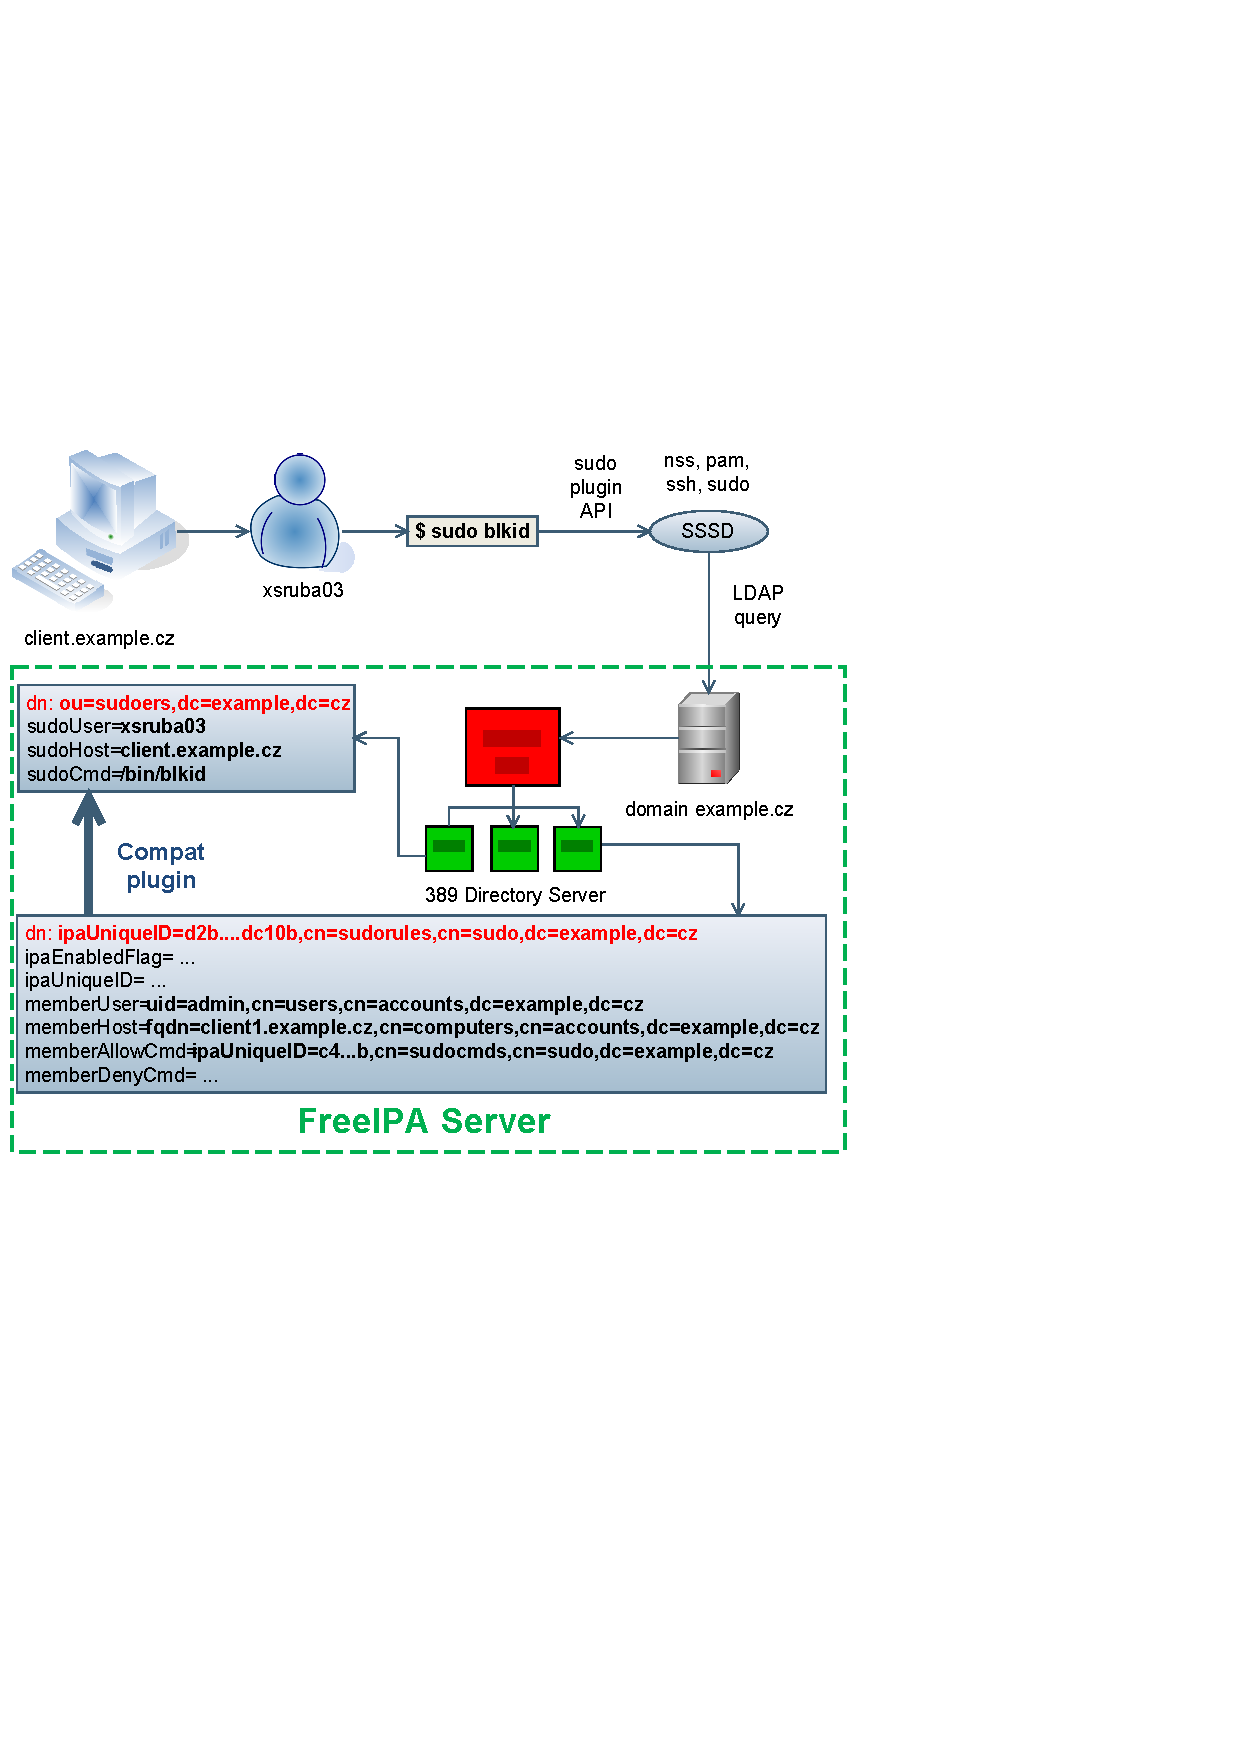
\includegraphics[scale=0.58]{img/1.pdf}
    \end{figure}
\end{frame}

\begin{frame}
    \frametitle{Purpose of my thesis}
    \begin{figure}
        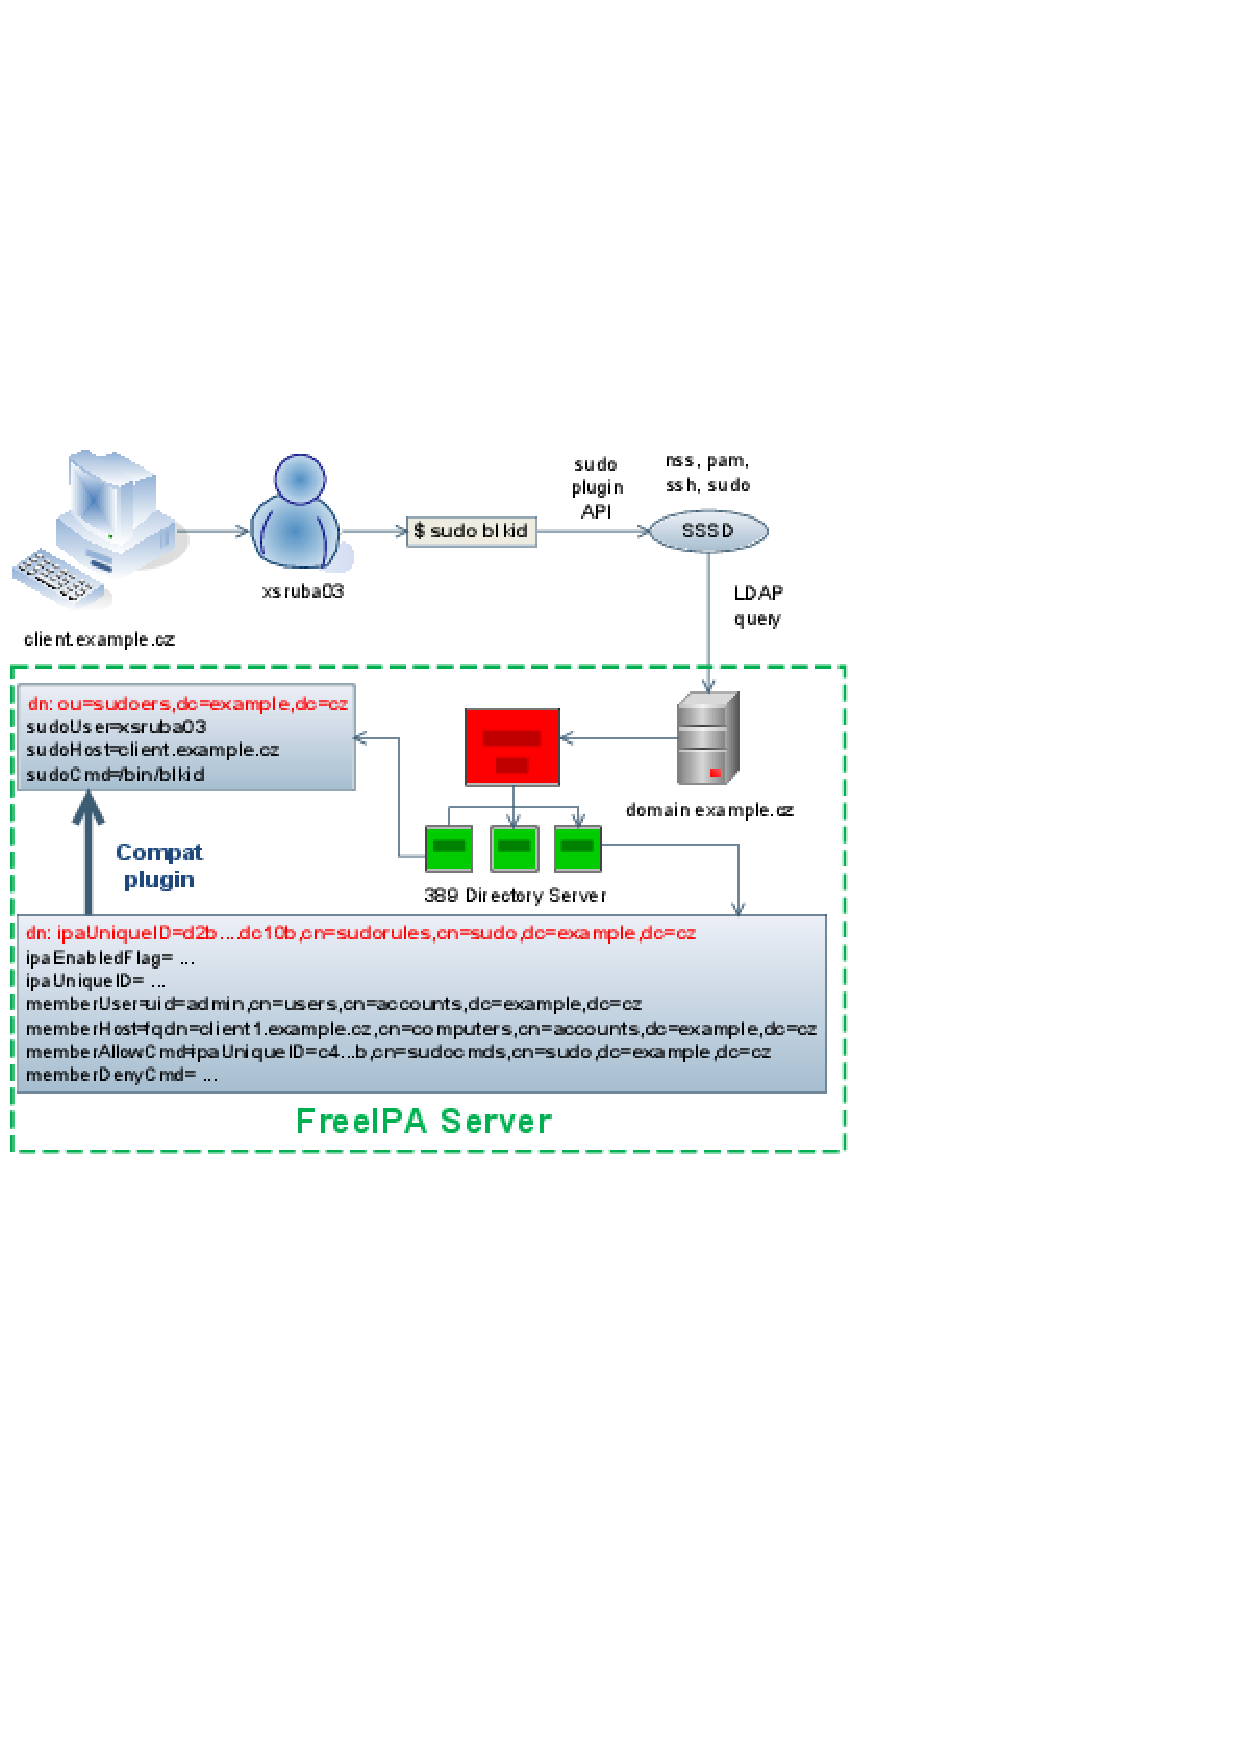
\includegraphics[scale=0.58]{img/2.pdf}
    \end{figure}
\end{frame}



\begin{frame}
    \frametitle{Current state}
    \begin{itemize}
        \item sudoers in ldap
        \item sudoers in FreeIPA
        \item sudoers in SSSD
        \item differences between sudo LDAP scheme and FreeIPA sudo scheme
        \item SSSD drawbacks
    \end{itemize}
\end{frame}

\begin{frame}
    \frametitle{Next steps}
    \begin{itemize}
        \item fix bugs from sssd's tickets
        \item design necessary changes
        \item feedback from developer's community
            \begin{itemize}
                \item implement designed changes
            \end{itemize}
        \item unit tests
    \end{itemize}
\end{frame}

\mode<presentation> {
    \begin{rhbg}
    \begin{frame}
    \vspace
    {\color{white}{\hfill \huge{The end}\hfill }}
    {\color{white}{\hfill Thank you for listening.\hfill}}
    \end{frame}
    \end{rhbg}
}

\begin{frame}[fragile]
    \frametitle{Benefits of the SSSD (System Security Services Daemo}
    \begin{itemize}
        \item client can connect into multiple domains
        \begin{itemize}
            \item each server can provide different kind of information
        \end{itemize}
        \item can detect disconnection from the network
        \item cache information about user, passwords, sudo rules
        \begin{itemize}
            \item cache stores only used data
            \item offline support
            \item cache entries expires
            \item no need of local account anymore
        \end{itemize}
    \end{itemize}
\end{frame}


\begin{frame}[fragile]
    \frametitle{Architecture of the SSSD}
    \begin{figure}
        \includegraphics[scale=0.20]{img/sssd-architecture.png}
    \end{figure}
\end{frame}

\begin{frame}[fragile]
    \frametitle{Why new LDAP scheme for sudo?}
    \begin{itemize}
        \item interconnection with IPA objects
        \item addition information (e.g. ipaRuleEnabled)
        \item more flexibility for ipa developers
    \end{itemize}
\end{frame}



\end{document}
